\documentclass[12pt,a4paper]{article}
\usepackage{amsmath,amscd,amsbsy,amssymb,latexsym,url,bm,amsthm}
\usepackage{epsfig,graphicx,subfigure}
\usepackage{enumitem,balance}
\usepackage{wrapfig}
\usepackage{mathrsfs,euscript}
\usepackage[usenames]{xcolor}
\usepackage{hyperref}
\usepackage[vlined,ruled,linesnumbered]{algorithm2e}
\usepackage{array}
\hypersetup{colorlinks=true,linkcolor=black}
\usepackage{attachfile}
\usepackage{listings}

\newtheorem{theorem}{Theorem}
\newtheorem{lemma}[theorem]{Lemma}
\newtheorem{proposition}[theorem]{Proposition}
\newtheorem{corollary}[theorem]{Corollary}
\newtheorem{exercise}{Exercise}
\newtheorem*{solution}{Solution}
\newtheorem{definition}{Definition}
\theoremstyle{definition}

\renewcommand{\thefootnote}{\fnsymbol{footnote}}

\newcommand{\postscript}[2]
 {\setlength{\epsfxsize}{#2\hsize}
  \centerline{\epsfbox{#1}}}

\renewcommand{\baselinestretch}{1.0}

\setlength{\oddsidemargin}{-0.365in}
\setlength{\evensidemargin}{-0.365in}
\setlength{\topmargin}{-0.3in}
\setlength{\headheight}{0in}
\setlength{\headsep}{0in}
\setlength{\textheight}{10.1in}
\setlength{\textwidth}{7in}
\makeatletter \renewenvironment{proof}[1][Proof] {\par\pushQED{\qed}\normalfont\topsep6\p@\@plus6\p@\relax\trivlist\item[\hskip\labelsep\bfseries#1\@addpunct{.}]\ignorespaces}{\popQED\endtrivlist\@endpefalse} \makeatother
\makeatletter
\renewenvironment{solution}[1][Solution] {\par\pushQED{\qed}\normalfont\topsep6\p@\@plus6\p@\relax\trivlist\item[\hskip\labelsep\bfseries#1\@addpunct{.}]\ignorespaces}{\popQED\endtrivlist\@endpefalse} \makeatother

\begin{document}
\noindent

%========================================================================
\noindent\framebox[\linewidth]{\shortstack[c]{
\Large{\textbf{Lab06-Linear Programming}}\vspace{1mm}\\
CS214-Algorithm and Complexity, Xiaofeng Gao, Spring 2021.}}
\begin{center}
\footnotesize{\color{red}$*$ If there is any problem, please contact TA Haolin Zhou.}

% Please write down your name, student id and email.
\footnotesize{\color{blue}$*$ Name: WendiChen  \quad Student ID: 519021910071 \quad Email: chenwendi-andy@sjtu.edu.cn}
\end{center}

\begin{enumerate}
    \item
    \textit{Hirschberg Algorithm.} Recall the \textbf{String Similarity} problem in class, in which we calculate the edit distance between two strings in a sequence alignment manner.
    \begin{enumerate}
    	\item
    	Implement the algorithm combining \textbf{dynamic programming} and \textbf{divide-and-conquer} strategy in C/C++. Analyze the time complexity of your algorithm. {\color{blue}(The template \emph{Code-SequenceAlignment.cpp} is attached on the course webpage)}.
    	
    	\item
    	Given $\alpha(x, y) = |ascii(x) - acsii(y)|$, where $ascii(c)$ is the ASCII code of character $c$, and $\delta=13$. Find the edit distance between the following two strings.
    	\begin{align*}
    		X[1..60]=&\ CMQHZZRIQOQJOCFPRWOUXXCEMYSWUJ\\
    		&\ TAQBKAJIETSJPWUPMZLNLOMOZNLTLQ	
    	\end{align*}
    	\begin{align*}
    		Y[1..50]=&\ SUYLVMUSDROFBXUDCOHAATBKN\\
    		&\ AAENXEVWNLMYUQRPEOCJOCIMZ
    	\end{align*}
    \end{enumerate}
    \begin{solution}
    ~
    \begin{enumerate}
        \item 
        Please refer to \emph{Code-SequenceAlignment.cpp}.\\
        Let $T(m,n)$ be the max running time of algorithm on strings of length $m$ and $n$. Then we will prove that $T(m,n) = O(mn)$. Actually, we have the recurrence, where finding index $q$ costs $O(mn)$
        \begin{align*}
            T(m,n) \leq T(q,\frac{n}{2})+T(m-q,\frac{n}{2}) +O(mn)
        \end{align*}
        According to the algorithm, we can choose a constant $c$ so that
        \begin{align*}
            \begin{split}
                T(m,2)&\leq cm\\
                T(2,n)&\leq cn\\
                T(m,n) &\leq cmn + T(q,\frac{n}{2})+T(m-q,\frac{n}{2})
            \end{split}
        \end{align*}
        Then we prove the statement by induction on n.\\
        For basis, when $n=2$, we have $T(m,2)\leq cm < 2cmn$.\\
        Then for every $n = 2^k,k>1$. We assume $T(m,\frac{n}{2})\leq cmn$ and get
        \begin{align*}
        \begin{split}
            T(m,n)&\leq T(q,\frac{n}{2})+T(m-q,\frac{n}{2})+cmn\\
            &\leq 2cq\frac{n}{2}+2c(m-q)\frac{n}{2}+cmn\\
            &= cqn+cmn-cqn+cmn\\
            &= 2 cmn
        \end{split}
        \end{align*}
        Thus, the time complexity is $O(mn)$.
        \item
        The running result of the program is shown below (Figure \ref{Fig-HirschbergAlgorithm}).
        \begin{figure}[htbp]
                \centering 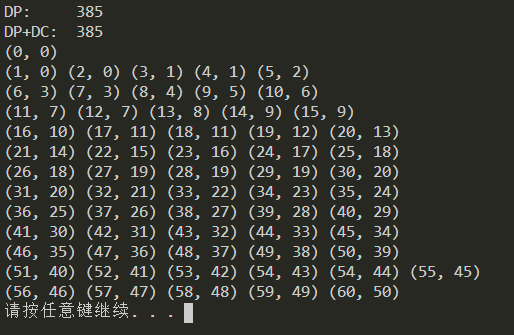
\includegraphics[width=0.6\textwidth]{Fig-HirschbergResult.png}
                \caption{Result of the Hirschberg Algorithm}\label{Fig-HirschbergAlgorithm}
        \end{figure}
    \end{enumerate}
    \end{solution}
    
    \item 
    \textit{Travelling Salesman Problem.} Given a list of cities and the distances between each pair of cities ($ G=(V,E,W) $), we want to find the shortest possible route that visits each city exactly once and returns to the origin city. Similar to \textbf{Maximum Independent Set} and \textbf{Dominating Set}, please turn the traveling salesman problem into an ILP form.  
    
    \textbf{Remark:} $ W $ is the set of weights corresponds to the edges that connecting adjacent cities.  
    
    \begin{solution}
    ~\\
    Suppose that $x_e$ is a 0-1 indicator of edge $e$, such that
    $$ x_e=\left\{
    \begin{aligned}
    & 1,&\quad \text{$e$ is selected in the route} \\
     & 0,&\quad \text{$e$ is not selected in the route}
    \end{aligned}
    \right.
    $$
    Then $\sum_{e\in E} x_e W_e$ denotes the length of the route, and thus we can formulate the following ILP:
    \begin{align*}
        \begin{split}
        & min \quad \sum_{e\in E} x_e W_e \\
        & s.t.\quad \sum_{e\in N(u)} x_e = 2 \quad \forall u\in V\\
        &\sum_{u\in V^{'}}\sum_{e\in N(u)} x_e < 2|V^{'}| \quad \forall V^{'} \subsetneq V\\
        & x_e \in \{0,1\} \quad \forall e\in E
        \end{split}
    \end{align*}
    where $N(u)$ denotes the set of edges that are connected to vertex $u$.
    \end{solution}
    
    \item
    \textit{Investment Strategy.} A company intends to invest $0.3$ million yuan in $2021$, with a proper combination of the following $3$ projects:
    \begin{itemize}
    \item \textbf{Project 1:} Invest at the beginning of a year, and can receive a $20\%$ profit of the investment in this project at the end of this year. Both the capital and profit can be invested at the beginning of next year;
    \item \textbf{Project 2:} Invest at the beginning of $2021$, and can receive a $50\%$ profit of the investment in this project at the end of $2022$. The investment in this project cannot exceed $0.15$ million dollars;
    \item \textbf{Project 3:} Invest at the beginning of $2022$, and can receive a $40\%$ profit of the investment in this project at the end of $2022$. The investment in this project cannot exceed $0.1$ million dollars.
    \end{itemize}
    Assume that the company will invest \emph{all} its money at the beginning of a year. Please design a scheme of investment in $2021$ and $2022$ which maximizes the overall sum of capital and profit at the end of $2022$.
    \begin{enumerate}
    \item
    Formulate a linear programming with necessary explanations.

    \item
    Transform your LP into its standard form and slack form.

    \item
    Transform your LP into its dual form.

    \item
    Use the simplex method to solve your LP.
    \end{enumerate}
    \begin{solution}
    ~
    \begin{enumerate}
        \item 
        During the whole process, we need to make decisions at two points in time--at the beginning of 2021 and at the beginning of 2022. At the beginning of 2021, we can divide the funds into two parts. One part for project 1 and the other part for project 2. Thus, we have $x_1+x_2 = 0.3$ and $x_2\leq 0.15$. Thus, at the beginning of 2022, all money we have make use of is $1.2x_1$. Similarly, we divide the money into two parts and have $x_3+x_4 = 1.2x_1$ and $x_4\leq 0.1$. So the overall sum of capital and profit at the end of 2022 is $1.5 x_2 + 1.2x_3+1.4x_4$. Of course, all $x_i$ should be positive. Thus, we have derived a LP:
        \begin{align*}
            \begin{split}
                max \quad f(x_2,x_3,x_4) &= 1.5 x_2 + 1.2x_3+1.4x_4\\
                s.t.\quad\quad\quad x_1+x_2 &= 0.3\\
                x_2 &\leq 0.15\\
                x_3+x_4 - 1.2x_1&= 0\\
                x_4 &\leq 0.1\\
                x_1,x_2,x_3,x_4&\ge 0
            \end{split}
        \end{align*}
        \item
        We transform the $LP$ into its standard form first.
        \begin{align*}
            \begin{split}
                max \quad f(x_2,x_3,x_4) &= 1.5 x_2 + 1.2x_3+1.4x_4\\
                s.t.\quad\quad\quad x_1+x_2 &\leq 0.3\\
                -x_1-x_2 &\leq -0.3\\
                x_2 &\leq 0.15\\
                x_3+x_4 -1.2x_1&\leq 0\\
                -x_3-x_4 +1.2x_1&\leq 0\\
                x_4 &\leq 0.1\\
                x_1,x_2,x_3,x_4&\ge 0
            \end{split}
        \end{align*}
        Then we transform it into a slack form.
        \begin{align*}
            \begin{split}
                max \quad f(x_2,x_3,x_4) &= 1.5 x_2 + 1.2x_3+1.4x_4\\
                s.t.\quad\quad\quad x_1+x_2&= 0.3\\
                x_2+x_5 &= 0.15\\
                x_3+x_4 -1.2x_1&= 0\\
                x_4 +x_6&= 0.1\\
                x_1,x_2,x_3,x_4,x_5,x_6&\ge 0
            \end{split}
        \end{align*}
        \item
        We define six multipliers $y_1,y_2,y_3,y_4,y_5$ and $y_6$. And after that we get
        \begin{align*}
            \begin{split}
                &(y_1-y_2-1.2y_4+1.2y_5)x_1+(y_1-y_2+y_3)x_2+(y_4-y_5)x_3+(y_4-y_5+y_6)x_4\\
                &\leq 0.3y_1-0.3y_2+0.15y_3+0.1y_6
            \end{split}
        \end{align*}
        Then we derive the dual form.
        \begin{align*}
            \begin{split}
                min \quad\quad\quad\quad\quad\quad f(y_1,y_2,y_3,y_4)&=0.3y_1-0.3y_2+0.15y_3+0.1y_6\\
                s.t.\quad\quad\quad
                y_1-y_2-1.2y_4+1.2y_5 &\ge0\\
                y_1-y_2+y_3&\ge 1.5\\
                y_4-y_5&\ge 1.2\\
                y_4-y_5+y_6&\ge 1.4\\
                y_1,y_2,y_3,y_4,y_5,y_6&\ge0
            \end{split}
        \end{align*}
        \item
        We set $x_1,x_5,x_6,x_7$ as basic variables. Thus the slack form can be written as
        \begin{align*}
            \begin{split}
                max \quad f(x_2,x_3,x_4) &= 1.5 x_2 + 1.2x_3+1.4x_4\\
                s.t.\quad\quad\quad 0.3-x_2&= x_1\\
                0.15-x_2 &= x_5\\
                0.36-1.2x_2 -x_4-x_3&=x_7\\
                0.1 -x_4 &= x_6\\
                x_1,x_2,x_3,x_4,x_5,x_6,x_7&\ge 0
            \end{split}
        \end{align*}
        The basic solution is $\overline{x} = (0.3,0,0,0,0.15,0.1,0.36)$. Next, we choose the nonbasic variable $x_2$ and $0.15-x_2=x_5$ is the tightest constraint for $x_2$, so we transform it into $0.15-x_5=x_2$. The nonbasic variables become $x_3,x_4,x_5$.
        \begin{align*}
            \begin{split}
                max \quad f(x_5,x_3,x_4) &= 1.5(0.15-x_5) + 1.2x_3+1.4x_4\\
                s.t.\quad\quad\quad 0.15+x_5&= x_1\\
                0.15-x_5 &= x_2\\
                0.18+1.2x_5 -x_4-x_3&=x_7\\
                0.1 -x_4 &= x_6\\
                x_1,x_2,x_3,x_4,x_5,x_6,x_7&\ge 0
            \end{split}
        \end{align*}
        And we get $\overline{x} = (0.15,0.15,0,0,0,0.1,0.18)$. Similarly, we choose the nonbasic variable $x_4$ and $0.1 -x_4 = x_6$ is the tightest constraint. And the nonbasic variable becomes $x_3,x_5,x_6$.
        \begin{align*}
            \begin{split}
                max \quad f(x_5,x_3,x_6) &= 1.5(0.15-x_5) + 1.2x_3+1.4(0.1-x_6)\\
                s.t.\quad\quad\quad 0.15+x_5&= x_1\\
                0.15-x_5 &= x_2\\
                0.08+1.2x_5 +x_6-x_3&=x_7\\
                0.1 -x_6 &= x_4\\
                x_1,x_2,x_3,x_4,x_5,x_6,x_7&\ge 0
            \end{split}
        \end{align*}
        And we get $\overline{x} = (0.15,0.15,0,0.1,0,0,0.08)$. At last, we have $0.08+1.2x_5 +x_6-x_7=x_3$. So, we have to max $f(x_5,x_6,x_7) = 1.5(0.15-x_5) + 1.2(0.08+1.2x_5 +x_6-x_7)+1.4(0.1-x_6) = 0.461-0.06x_5-0.2x_6-1.2x_7$. Now all coefficients are negative. The optimal solution is $\overline{x} = (0.15,0.15,0.08,0.1,0,0,0)$. The overall sum of capital and profit is 0.461 million yuan.
    \end{enumerate}
    \end{solution}
    \item
    \textit{Factory Production.} An engineering factory makes seven products (PROD 1 to PROD 7) on the following machines: four grinders, two vertical drills, three horizontal drills, one borer and one planer. Each product yields a certain contribution to profit (in \pounds/unit). These quantities (in \pounds/unit) together with the unit production times (hours) required on each process are given below. A dash indicates that a product does not require a process.

    \begin{table}[htbp]
      \scriptsize
      \centering
      \renewcommand\arraystretch{1.1}
      \begin{tabular}{m{0.18\textwidth} m{0.07\textwidth}<{\centering} m{0.07\textwidth}<{\centering} m{0.07\textwidth}<{\centering} m{0.07\textwidth}<{\centering} m{0.07\textwidth}<{\centering} m{0.07\textwidth}<{\centering} m{0.07\textwidth}<{\centering}}
      \hline
       & \textbf{PROD 1} & \textbf{PROD 2} & \textbf{PROD 3} & \textbf{PROD 4} & \textbf{PROD 5} & \textbf{PROD 6} &  \textbf{PROD 7} \\\hline
      Contribution to profit & 10 & 6 & 8 & 4 & 11 & 9 & 3 \\
      Grinding & 0.5 & 0.7 & - & - & 0.3 & 0.2 & 0.5 \\
      Vertical drilling & 0.1 & 0.2 & - & 0.3 & - & 0.6 & - \\
      Horizontal drilling & 0.2 & - & 0.8 & - & - & - & 0.6 \\
      Boring & 0.05 & 0.03 & - & 0.07 & 0.1 & - & 0.08 \\
      Planing & - & - & 0.01 & - & 0.05 & - & 0.05 \\
      \hline
      \end{tabular}
    \end{table}

    There are marketing limitations on each product in each month, given in the following table:

    \begin{table}[htbp]
      \scriptsize
      \centering
      \renewcommand\arraystretch{1.1}
      \begin{tabular}{m{0.1\textwidth} m{0.07\textwidth}<{\centering} m{0.07\textwidth}<{\centering} m{0.07\textwidth}<{\centering} m{0.07\textwidth}<{\centering} m{0.07\textwidth}<{\centering} m{0.07\textwidth}<{\centering} m{0.07\textwidth}<{\centering}}
      \hline
       & \textbf{PROD 1} & \textbf{PROD 2} & \textbf{PROD 3} & \textbf{PROD 4} & \textbf{PROD 5} & \textbf{PROD 6} &  \textbf{PROD 7} \\\hline
      January & 500 & 1000 & 300 & 300 & 800 & 200 & 100 \\
      February & 600 & 500 & 200 & 0 & 400 & 300 & 150 \\
      March & 300 & 600 & 0 & 0 & 500 & 400 & 100 \\
      April & 200 & 300 & 400 & 500 & 200 & 0 & 100 \\
      May & 0 & 100 & 500 & 100 & 1000 & 300 & 0 \\
      June & 500 & 500 & 100 & 300 & 1100 & 500 & 60 \\
      \hline
      \end{tabular}
    \end{table}

    It is possible to store up to 100 of each product at a time at a cost of \pounds0.5 per unit per month (charged at the end of each month according to the amount held at that time). There are no stocks at present, but it is desired to have a stock of exactly 50 of each type of product at the end of June. The factory works six days a week with two shifts of 8h each day. It may be assumed that each month consists of only 24 working days. Each machine must be down for maintenance in one month of the six. No sequencing problems need to be considered.

    When and what should the factory make in order to maximize the total net profit?

    \begin{enumerate}
    \item
    Use \emph{CPLEX Optimization Studio} to solve this problem. Describe your model in \emph{Optimization Programming Language} (OPL). Remember to use a separate data file (.dat) rather than embedding the data into the model file (.mod).

    \item
    Solve your model and give the following results.
    \begin{enumerate}
    \item
    For each machine:
    \begin{enumerate}
    \item
    the month for maintenance.
    \end{enumerate}
    \item
    For each product:
    \begin{enumerate}
    \item
    The amount to make in each month.
    \item
    The amount to sell in each month.
    \item
    The amount to hold at the end of each month.
    \end{enumerate}
    \item
    The total selling profit.
    \item
    The total holding cost.
    \item
    The total net profit (selling profit minus holding cost).
    \end{enumerate}
    \end{enumerate}
    \textbf{Remark:} You can choose to use the attached .dat file or write it yourself. 
    \begin{solution}
    ~
    \begin{enumerate}
        \item 
        Please refer to \emph{model.mod} and \emph{FactoryPlanning.dat}.
        \item
        We assume that every unit of product for making, selling or storing is integer.
        \begin{enumerate}
            \item
            \begin{enumerate}
                \item 
                ~
                \begin{table}[htbp]
          \scriptsize
          \centering
          \renewcommand\arraystretch{1.1}
          \begin{tabular}{m{0.1\textwidth} m{0.07\textwidth}<{\centering} m{0.07\textwidth}<{\centering} m{0.07\textwidth}<{\centering} m{0.07\textwidth}<{\centering} m{0.07\textwidth}<{\centering}}
          \hline
           & \textbf{Grinders} & \textbf{Vertical Drills} & \textbf{Horizontal Drills} & \textbf{Borer} & \textbf{Planner}  \\\hline
          January & 0 & 0 & 1 & 0 & 0   \\
          February & 0 & 1 & 0 & 0 & 0   \\
          March & 0 & 0 & 0 & 0 & 0   \\
          April & 4 & 1 & 2 & 1 & 1  \\
          May & 0 & 0 & 0 & 0 & 0 \\
          June & 0 & 0 & 0 & 0 & 0  \\
          \hline
          \end{tabular}
        \end{table}
        \end{enumerate}
        
        \item
        \begin{enumerate}
            \item 
            ~
                \begin{table}[htbp]
              \scriptsize
              \centering
              \renewcommand\arraystretch{1.1}
              \begin{tabular}{m{0.1\textwidth} m{0.07\textwidth}<{\centering} m{0.07\textwidth}<{\centering} m{0.07\textwidth}<{\centering} m{0.07\textwidth}<{\centering} m{0.07\textwidth}<{\centering} m{0.07\textwidth}<{\centering} m{0.07\textwidth}<{\centering}}
              \hline
               & \textbf{PROD 1} & \textbf{PROD 2} & \textbf{PROD 3} & \textbf{PROD 4} & \textbf{PROD 5} & \textbf{PROD 6} &  \textbf{PROD 7} \\\hline
              January & 500 & 1000 & 300 & 300 & 800 & 200 & 100 \\
              February & 600 & 500 & 200 & 0 & 400 & 300 & 150 \\
              March & 400 & 700 & 100 & 100 & 600 & 400 & 200 \\
              April & 0 & 0 & 0 & 0 & 0 & 0 & 0 \\
              May & 0 & 100 & 500 & 100 & 1000 & 300 & 0 \\
              June & 550 & 550 & 150 & 350 & 1150 & 550 & 110 \\
              \hline
              \end{tabular}
            \end{table}
            \item 
            ~
                \begin{table}[htbp]
              \scriptsize
              \centering
              \renewcommand\arraystretch{1.1}
              \begin{tabular}{m{0.1\textwidth} m{0.07\textwidth}<{\centering} m{0.07\textwidth}<{\centering} m{0.07\textwidth}<{\centering} m{0.07\textwidth}<{\centering} m{0.07\textwidth}<{\centering} m{0.07\textwidth}<{\centering} m{0.07\textwidth}<{\centering}}
              \hline
               & \textbf{PROD 1} & \textbf{PROD 2} & \textbf{PROD 3} & \textbf{PROD 4} & \textbf{PROD 5} & \textbf{PROD 6} &  \textbf{PROD 7} \\\hline
              January & 500 & 1000 & 300 & 300 & 800 & 200 & 100 \\
              February & 600 & 500 & 200 & 0 & 400 & 300 & 150 \\
              March & 300 & 600 & 0 & 0 & 500 & 400 & 100 \\
              April & 100 & 100 & 100 & 100 & 100 & 0 & 100 \\
              May & 0 & 100 & 500 & 100 & 1000 & 300 & 0 \\
              June & 500 & 500 & 100 & 300 & 1100 & 500 & 60 \\
              \hline
              \end{tabular}
            \end{table}
            \item 
            ~
                \begin{table}[!htbp]
              \scriptsize
              \centering
              \renewcommand\arraystretch{1.1}
              \begin{tabular}{m{0.1\textwidth} m{0.07\textwidth}<{\centering} m{0.07\textwidth}<{\centering} m{0.07\textwidth}<{\centering} m{0.07\textwidth}<{\centering} m{0.07\textwidth}<{\centering} m{0.07\textwidth}<{\centering} m{0.07\textwidth}<{\centering}}
              \hline
               & \textbf{PROD 1} & \textbf{PROD 2} & \textbf{PROD 3} & \textbf{PROD 4} & \textbf{PROD 5} & \textbf{PROD 6} &  \textbf{PROD 7} \\\hline
              January & 0 & 0 & 0 & 0 & 0 & 0 & 0 \\
              February & 0 & 0 & 0 & 0 & 0 & 0 & 0 \\
              March & 100 & 100 & 100 & 100 & 100 & 0 & 100 \\
              April & 0 & 0 & 0 & 0 & 0 & 0 & 0 \\
              May & 0 & 0 & 0 & 0 & 0 & 0 & 0 \\
              June & 50 & 50 & 50 & 50 & 50 & 50 & 50 \\
              \hline
              \end{tabular}
            \end{table}
            
        \end{enumerate}
        \newpage
        \item
        The total selling profit is 109330\pounds.
        \item
        The total holding cost is 475\pounds.
        \item
        The total net profit is 108855\pounds.
        \end{enumerate}
    \end{enumerate}

    \end{solution}

\end{enumerate}
\newpage
\vspace{20pt}

{\noindent\large\textbf{Appendix}}
\begin{enumerate}
	\item [\textbf{A.}]
	\textbf{FactoryPlanning.dat}
	\attachfile{FactoryPlanning.dat}
	\lstset{
		language=C,
		tabsize=2,
		basicstyle=\footnotesize\ttfamily,
		columns=fullflexible,
		keywordstyle=\color{blue},
		numbers=left,
		numberstyle=\scriptsize\ttfamily,
		frame=single
	}
	\begin{lstlisting}
		NbMonths = 6;
		
		Prod = {Prod1, Prod2, Prod3, Prod4, Prod5, Prod6, Prod7};
		Process = {Grind, VDrill, HDrill, Bore, Plane};
		
		// profitProd[j] is profit per unit for product j
		ProfitProd = [10 6 8 4 11 9 3];
		
		// processProd[i][j] gives hours of process i required by product j
		ProcessProd = [[0.5  0.7  0.0  0.0  0.3  0.2 0.5 ]
		[0.1  0.2  0.0  0.3  0.0  0.6 0.0 ]
		[0.2  0.0  0.8  0.0  0.0  0.0 0.6 ]
		[0.05 0.03 0.0  0.07 0.1  0.0 0.08]
		[0.0  0.0  0.01 0.0  0.05 0.0 0.05]];
		
		// marketProd[i][j] gives marketing limitation on product j for month i
		MarketProd = [[500 1000 300  300 800  200 100]
		[600 500  200  0   400  300 150]
		[300 600  0    0   500  400 100]
		[200 300  400  500 200  0   100]
		[0   100  500  100 1000 300 0  ]
		[500 500  100  300 1100 500 60 ]];
		
		CostHold  = 0.5;
		StartHold = 0;
		EndHold   = 50;
		MaxHold   = 100;
		
		// process capacity
		HoursMonth = 384; // 2 eight hour shifts per day, 24 working days per month;
		
		// number of each type of machine
		NumProcess = [4 2 3 1 1];
		
		// how many machines must be down over 6 month period
		NumDown = [4 2 3 1 1];
	\end{lstlisting}
\end{enumerate}

\textbf{Remark:} You need to include your .cpp, .mod, .dat, .pdf and .tex files in your uploaded .zip file.

%========================================================================
\end{document}
